%%
%%
\documentclass[12pt]{book}
\usepackage{amsfonts,amssymb,amsmath,amsthm}
\usepackage{graphicx}
\usepackage{hyperref}
\usepackage{boxedminipage}
\usepackage{geometry}
\usepackage{array}
\usepackage{enumitem}

\newcolumntype{C}[1]{>{\centering\let\newline\\\arraybackslash\hspace{0pt}}m{#1}}

\setlength{\textheight}{10in}
\setlength{\textwidth}{7.4in}
\setlength{\topmargin}{-0.75in}
\setlength{\oddsidemargin}{-0.5in}
\setlength{\evensidemargin}{-0.5in}
\setlength{\parskip}{0.15in}
\setlength{\parindent}{0in}


\begin{document}


\vspace{-1.0in}\begin{center}
\Large{MCV4U : Calculus and Vectors}\\
\Large{MCV4UR : Advanced Placement Calculus and Vectors }

\Large{Assignment \#1}


\end{center}

%\medskip

\vspace{0.015in}\hrulefill\ 

\textbf{Reference Declaration} %  Fill in your Reference Declarations in this section before your submit your assignment.

Complete the Reference Declaration section below in order for your assigment to be graded.

If you used any references beyond the course text and lectures (such as other texts, discussions with colleagues or online resources), indicate this information in the space below.  If you did not use any aids, state this in the space provided. 

Be sure to cite appropriate theorems throughout your work. You may use shorthand for well-known theorems like the FT, RRT, MVT, IVT, etc. 

Note: Your submitted work must be \textbf{your original work}. 

Family Name: Wong\\%Family Name Here
First Name: Max %First Name Here

Declared References: 

% Type your references here.
% You can use as many lines as required.

\vspace{0.015in}\hrulefill\ 

\newpage

% INSTRUCTIONS SECTION
\section*{Instructions}

\begin{center}
\setlength{\fboxrule}{2pt}
\begin{boxedminipage}{6.5in}
1.	Organize and express complete, effective and concise responses to each problem.\\
2.	Use appropriate mathematical conventions and notation wherever possible.\\
3.	Provide logical reasoning for your arguments and cite any relevant theorems. \\
4.  The quality of your communication will be heavily weighted.
\end{boxedminipage}
\end{center} 

% EVALUATION SECTION
\section*{Evaluation}

% LEARNING EXPECTATION(S)
\begin{itemize}
\item Students will demonstrate an understanding of limits and apply them to solve problems.
\end{itemize}

% RUBRIC
\begin{tabular}{| C{2in} | C{1in} | C{1in} | C{1in} | C{1in} |}
\hline
\textbf{Criteria} & \textbf{Level 1} & \textbf{Level 2} & \textbf{Level 3} & \textbf{Level 4} \\
\hline
\emph{Understanding of Mathematical Concepts} & Demonstrates limited understanding & Demonstrates some understanding & Demonstrates considerable understanding & Demonstrates thorough understanding of concepts \\
\hline
\emph{Selecting Tools and Strategies} & Selects and applies appropriate tools and strategies, with major errors, omissions, or mis-sequencing & Selects and applies appropriate tools and strategies, with minor errors, omissions, or mis-sequencing & Selects and applies appropriate tools and strategies accurately, and in a logical sequence & Selects and applies appropriate and efficient tools and strategies accurately to create mathematically elegant solutions \\
\hline
\emph{Reasoning and Proving} & Inconsistently or erroneously employs logic to develop and defend statements & Statements are developed and defended with some omissions or leaps in logic & Frequently develops and defends statements with reasonable logical justification & Consistently develops and defends statements with sophisticated and/or complete logical justification \\
\hline
\emph{Communicating} & Expresses and organizes mathematical thinking with limited effectiveness & Expresses and organizes mathematical thinking with some effectiveness & Expresses and organizes mathematical thinking with considerable effectiveness & Expresses and organizes mathematical thinking with a high degree of effectiveness \\
\hline
\end{tabular}

\pagebreak



%%%%%%%%%%%% PROBLEMS START HERE



\begin{enumerate}

%% PROBLEM 1
\item The sum $3-\dfrac{3}{10}+\dfrac{3}{100}-\dfrac{3}{1000} + \cdots + \dfrac{(-1)^k3}{10^k} + \cdots$ is closest to:
\begin{enumerate}
\item[(a)] $\dfrac{2}{e}$
\item[(b)] $2$
\item[(c)] $e$
\item[(d)] $e^2$
\end{enumerate}

%% PROBLEM 2
\item The value of $\lim_{x\to a}\limits \dfrac{x-a}{\sqrt{x} - \sqrt{a}}$ is:
\begin{enumerate}
\item[(a)] $2a$
\item[(b)] $2\sqrt{a}$
\item[(c)] $\sqrt{2a}$
\item[(d)] $a$
\end{enumerate}

%% PROBLEM 3
\item If $\lim_{x\to c}\limits f(x) = L$ where $L \in \mathbb{R}$ then which of the following must be true?
\begin{enumerate}
\item[(a)] $f$ is defined at $x=c$
\item[(b)] $f$ is continuous at $x=c$
\item[(c)] $f(c) = L$
\item[(d)] None of the above
\end{enumerate}

%% PROBLEM 4
\item Given $f$ is continuous on $[-2,6]$, if $f(-2)=7$ and $f(6)=-1$ then the Intermediate Value Theorem guarantees that:
\begin{enumerate}
\item[(a)] $f(0)=0$
\item[(b)] $f(c)=2$ for at least one value of $c \in [-2,6]$
\item[(c)] $f(c)=0$ for at least one value of $c \in [-1,7]$
\item[(d)] $\forall x \in [-2,6], -1 \le f(x) \le 7$
\end{enumerate}

%% PROBLEM 5
\item The value of $\lim_{x\to 0}\limits \dfrac{\sin(4x)}{2x}$ is:
\begin{enumerate}
\item[(a)] $0$
\item[(b)] $0.5$
\item[(c)] $1$
\item[(d)] $2$
\end{enumerate}

%% PROBLEM 6
\item The value of $\lim_{x\to -\infty}\limits \dfrac{\sqrt{8x^2 - 4x}}{x+2}$ is:
\begin{enumerate}
\item[(a)] $-\infty$
\item[(b)] $-2\sqrt{2}$
\item[(c)] $4$
\item[(d)] $2\sqrt{2}$
\end{enumerate}


\newpage

%% PROBLEM 7
\item The value of $k$ such that $f(x) = \begin{cases} 
      x^2 + 2 & : x \le -1 \\
      kx+4 & : x>-1 \\
   \end{cases}$ is continuous on $\mathbb{R}$ is: 
\begin{enumerate}
\item[(a)] $-3$
\item[(b)] $-1$
\item[(c)] $1$
\item[(d)] $3$
\end{enumerate}

%% PROBLEM 8
\item For what value of $a$ is the function $f(x) = \dfrac{x^2 - 3x}{x-a}$ continuous on $\mathbb{R}$?
\begin{enumerate}
\item[(a)] $-3$
\item[(b)] $-1$
\item[(c)] $3$
\item[(d)] There does not exist a value of $a$ such that $f$ is continuous on $\mathbb{R}$.
\end{enumerate}

%% PROBLEM 9
\item The value of $\lim_{x\to 0}\limits \dfrac{e^{ax} \sin(bx) \tan(cx)}{x^2}$, where $a,b,c \in \mathbb{R}\setminus\{0\}$ is:
\begin{enumerate}
\item[(a)] $\frac{a}{bc}$
\item[(b)] $bc$
\item[(c)] $\frac{ab}{c}$
\item[(d)] $ab$
\end{enumerate}

%% PROBLEM 10
\item The value of $\lim_{x\to 0}\limits x^3 \sin\left(\dfrac{1}{x}\right)$ is:
\begin{enumerate}
\item[(a)] $-1$
\item[(b)] $0$
\item[(c)] $1$
\item[(d)] nonexistent
\end{enumerate}

\newpage

\section*{Multiple Choice Answers}

\begin{enumerate}[label={\arabic*.}]
\item C
\item B
\item D
\item B
\item D
\item D
\item C
\item C
\item B
\item B
\end{enumerate}

Fill in your responses to the multiple choice questions above. Be sure to use capital letters.

\newpage

%% PROBLEM 11
\item If $f(x) = 3x^3 - 2x + 1$ then \textbf{determine} $f'(x)$ from \emph{First Principles} by using the definition of the derivative.


%% I would recommend sandwiching your solution to every problem between the kind of structure I have provided below re: initial \vspace, the Solution: heading and the ending \vspace.
\vspace{0.3cm} 
\textbf{Solution To Question 11:}\\
\\
Given the function $f(x) = 3x^2-2x+1$, we can solve for $f'(x)$ using the first principal 
definition of the derivative.

\addtolength{\jot}{1em}
\begin{align*}
    f'(x) &= \lim_{h \to 0} \dfrac{f(x+h)-f(x)}{h} && \text{First Principle Definition} \\
    f'(x) &= \lim_{h \to 0} \dfrac{(3(x+h)^2 - 2(x+h) + 1) - (3x^2-2x+1)}{h} && \text{Implement f(x) with x+h and x} \\
    f'(x) &= \lim_{h \to 0} \dfrac{3(x^2+2hx+h^2) - (2x+2h) + 1 - 3x^2+2x-1}{h} && \text{Expand and Simplify} \\
    f'(x) &= \lim_{h \to 0} \dfrac{3x^2+6hx+3h^2 - 2x-2h + 1 - 3x^2+2x-1}{h} \\
    f'(x) &= \lim_{h \to 0} \dfrac{6hx+3h^2-2h}{h} \\
    f'(x) &= \lim_{h \to 0} \dfrac{h(6x+3h-2)}{h} && \text{Factor h} \\
    f'(x) &= \lim_{h \to 0} 6x+3h-2 && \text{Simplify, Cross out h} \\
    f'(x) &= 6x-2 && \text{Apply Limit} \\
\end{align*}

$$\boxed{\text{Therefore, using the first principles we find that the derivative of f(x) is 6x-2.}}$$

\vspace{0.3cm}


\newpage


%% PROBLEM 12
\item \textbf{Evaluate} $\lim_{t\to 0}\limits \left(\dfrac{1}{t\sqrt{1+t}} - \dfrac{1}{t}\right)$ or assert that it does not exist and provide evidence to support your conclusion.

\vspace{0.3cm} 
\textbf{Solution To Question 12:}\\
 Your solution starts here.
\vspace{0.3cm}

\newpage

%% PROBLEM 13
\item \textbf{Evaluate} $\lim_{x\to 0}\limits \dfrac{\sqrt[3]{1+cx}-1}{x}$ where $c \in \mathbb{R^*}$.

\vspace{0.3cm} 
\textbf{Solution To Question 13:}\\
 Your solution starts here.
\vspace{0.3cm}

\newpage


%% PROBLEM 14
\item The figure shows a point $P$ on the parabola $y=x^2$ and the point $Q$ where the perpendicular bisector of $OP$ intersects the y-axis. As $P$ approaches the origin along the parabola, what happens to $Q$? Does it have a limiting position? If so, \textbf{determine} the limiting position of $Q$. 

\vspace{0.3cm} 
\textbf{Solution To Question 14:}\\
 Your solution starts here.
\vspace{0.3cm}


\newpage
\vspace{4cm}
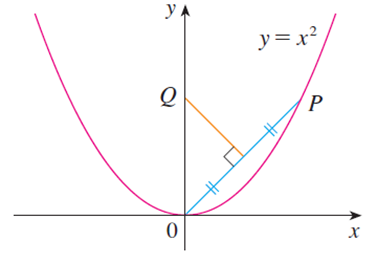
\includegraphics[width=\linewidth]{parabola.png}
%% WHEN YOU HAND IN YOUR WORK YOU CAN REMOVE THE IMAGE BY DELETING THE ABOVE TWO LINES


\newpage



\end{enumerate}
\end{document} 
